\documentclass{llncs}
\usepackage[utf8]{inputenc}
\usepackage{mathtools}
\usepackage{amsmath}

\DeclarePairedDelimiter{\ceil}{\lceil}{\rceil}
\DeclarePairedDelimiter{\floor}{\lfloor}{\rfloor}
\newtheorem{observation}{\textbf{Observation}}


\usepackage{graphicx} \usepackage{amssymb} \usepackage{mathtools}
\usepackage{amsmath}
\usepackage{algorithmic}
\usepackage[section]{algorithm}
\usepackage{authblk}
\usepackage{color}
\usepackage{textcomp}
\usepackage{tikz}		

\pagestyle{plain}

\begin{document}

\title{Improved approximation algorithm for Fault-Tolerant Facility Placement}

\author{Bartosz Rybicki\thanks{Research supported by NCN 2012/07/N/ST6/03068 grant} \and Jaroslaw Byrka\\ \{bry, jby\}@ii.uni.wroc.pl}

\institute{Institute of Computer Science\\ University of Wrocław, Poland}

\maketitle

\begin{abstract}
We consider the Fault-Tolerant Facility Placement problem (), which is a generalization of the classical Uncapacitated Facility Location problem (). In the  problem we have a set of clients  and a set of facilities . Each facility  can be opened many times. For each opening of facility  we pay . Our goal is to connect each client  with  open facilities in a way that minimizes the total cost of open facilities and established connections. 

In a series of recent papers  was essentially reduced to  and then to  showing it could be approximated with ratio . In this paper we show that  can actually be approximated even better. We consider approximation ratio as a function of  (minimum requirement of a client). With increasing  the approximation ratio of our algorithm  converges to one. Furthermore, for  the value of  is less than 1.463 (hardness of approximation of ). We also show a lower bound of 1.278 for the approximability of the Fault-Tolerant Facility Location problem () for arbitrary . Already for  we obtain that  can be approximated with ratio 1.275, showing that under standard complexity theoretic assumptions  is strictly better approximable than . 
\end{abstract}

\newpage

\section{Introduction}
In the Fault-Tolerant Facility Placement problem, we are given a set  of locations where facilities may be opened (each  costs  and can be opened many times) and a set  of clients. Each  has connection requirement . Our goal is to open a subset of facilities (possibly many copies of some facilities) and connect each client  with  open facilities, such that the total cost of connections and opened facilities is as small as possible. In this paper we consider the metric version of the problem where the connection costs satisfy the triangle inequality.

It is easy to see that the classical  problem is a special case of  with all  . On the other hand, if no facility can be open more than once, then the problem becomes the Fault-Tolerant Facility Location problem (FTFL), in which the demands cannot exceed the number of facilities. 

Facility location problems are typically APX-hard and there exist constant factor approximation algorithms assuming metric connection costs. Shmoys, Tardos and Aardal \cite{Tardos} gave the first constant factor -approximation algorithm based on LP-rounding. Later Chudak and Shmoys \cite{Chudak} obtained -approximation by marginal-preserving randomized  rounding of facility openings, which has became standard for facility location problems. The long line of results for UFL includes a primal-dual algorithm JMS \cite{Jain}, which was then combined with a scaled version of \cite{Chudak} in a work of Byrka and Aardal \cite{Aardal}. The currently best known ration of 1.488 was obtained by Shi Li \cite{ShiLi} by further randomizing the algorithm from \cite{Aardal}. Many techniques developed for  can be directly applied to  which was shown in \cite{Yan}.

First constant factor approximation algorithm for the closely related  problem was given by Guha, Meyerson and Munagala \cite{Meyerson}. Next Swamy and Shmoys  improved the ratio to 2.076, see~\cite{Swamy}. More recently Byrka, Srinivasan and Swamy~\cite{ftfl_1725} improved the ratio to 1.725 using dependent rounding~\cite{Aravind} and laminar clustering. Moreover it is shown in~\cite{Swamy} that JMS algorithm can be adapted to  with uniform requirements of clients.

 was first studied by Xu and Shen \cite{Xu} and next by Yan and Chrobak who first obtained a -approximation algorithm~\cite{Yan_316}, and later improved the ratio to ~\cite{Yan}.

\subsection{Our contribution}

We extend the work of Yan and Chrobak~\cite{Yan} and propose an algorithm with approximation ratio being a decreasing function of the minimal requirement . Our solution benefits from requirements of clients being bigger than one. Instead of considering a client  as  distinct clients with unit demand we raven on this multiplicity and use Poisson distribution to estimate the expected number of useful facilities which will be open in a set of a particular volume. We consider both cases: uniform and non-uniform requirements of clients, and obtain the following approximation ratios: 

\begin{center}
  \begin{tabular}{ c | c | c | c | c | c | c | c | c | c | c }
     & 1 & 2 & 3 & 4 & 5 & 6 & 7 & 8 & 9 & 10 \\ \hline
    non-uniform & 1.515 & 1.439 & 1.338 & 1.275 & 1.234 & 1.207 & 1.187 & 1.171 & 1.159 & 1.149 \\ \hline
    uniform & 1.488 & 1.410 & 1.329 & 1.272 & 1.234 & 1.207 & 1.187 & 1.171 & 1.159 & 1.149 \\
  \end{tabular}
\end{center}

We also prove a lower bound of 1.278 on the approximability of Fault-Tolerant Facility Location (where at most one facility may be opened in each location) for arbitrarily large . 

\begin{observation}
 Lower bound for , of value , is bigger than  for . Moreover for   is easier than 
\end{observation}

Note that  for  (in both uniform and non-uniform case) is bounded by , which is smaller than our lower bound for .

\section{The LP formulation}
\label{the_lp_section}

Consider the following standard LP relaxation of .



An optimal solution of the above LP is denoted by a pair . Using these variables we express the total facility cost as  and the connection cost of each client  as . Summing over all clients gives the total connection cost  of the LP solution. The cost of  denoted by  is a lower bound on the cost of an optimal integral solution denoted by .

We say that a solution is complete if for each client  and each facility  we have . Detailed description of a technique called \textit{facility splitting}, which yields complete solutions, can be found in \cite{Sviridenko}. The splitting algorithm takes as input a solution of the LP and outputs a complete solution of the same cost to a larger, but equivalent instance of the problem. For clarity of a presentation, throughout the paper, we simply assume that all fractional solutions are complete.

\begin{definition}
 The volume of a set , denoted by  is the sum of facility openings in this set, i.e., .
\end{definition}

One of the problems with input instances is possibly non-polynomial demand of some clients. In \cite{Yan} we can find an elegant reduction of such instance to instances with requirements bounded by . In Section \ref{r_vs_apx} we give an algorithm which generalizes this reduction. Our algorithm also reduces the input instance to an instance with polynomial demands of clients, but we also care not to reduce the requirements of clients too much.

\section{Algorithm for }
The following algorithm  is parametrized by a real constant .
\begin{algorithm}
  \caption{}
\begin{algorithmic}[1]
 \STATE formulate and solve the LP (\ref{lp_ufl:goal})-(\ref{lp_ufl:non_negative}), get an optimal solution ;
 \STATE scale up facility opening by , then recompute values of  to obtain a minimum cost solution ;\\
 \STATE compute clustering for all clients;
 \STATE round facility opening variables using dependent rounding;
 \STATE connect each client  with  closest open facilities;
\end{algorithmic}
\end{algorithm}
Our final  is as follows: run algorithm  for each choice of , where . Select the best of the obtained solutions. Note that  is the number of different values of , each of them we use as a parameter of algorithm . In the computation of approximation ratios we use  equal 1000, but we will describe our results for a general n.

Scaling facility opening is an idea from \cite{Aardal}, it decreases average connection cost of each client, but increases total cost of opening facilities. In  we can open more than one facility in one location, so scaling does not cause problems with opening more than one facility in one place. The version of clustering which we use is very close to the one described in \cite{Chudak}. To round facility opening variables we use the randomized algorithm from \cite{Aravind}, called dependent rounding. Each step of the algorithm  is carefully described in the following sections.

\subsection{Scaling}

Let  denote the set of facilities with a positive flow from a client , i.e., facilities  with  in the optimal LP solution. 

Let . Suppose that all facilities are sorted in an order of non-decreasing distances from a client . Scaling all  variables by  divides the set of facilities  into two disjoint subsets: the set of close facilities of a client , denoted by , such that ;  and the distant facilities, denoted by , note that . Certainly for each  and  we have .

By  and  we denote the average distances to close, distant and all facilities in set , respectively. More formally:  By  we denote the maximal distance to a facility in , and by  we denote the average distance to  for ,  and . (see Fig.~\ref{partition_of_F_j})

\begin{figure}
  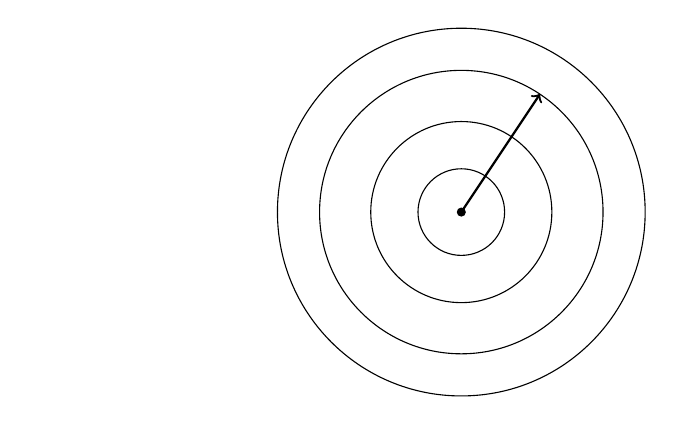
\begin{tikzpicture}
      \draw[fill=black] (6,.5) circle (0.05);
      \path (5.8, 0.4) node {};
      
      \draw (6,.5) circle (.55);
      \path (6.3, 0.5) node {};
      
      \draw (6,.5) circle (1.15);
      \path (6.85, 0.5) node {};
      
      \draw (6,.5) circle (1.8);
      \path (6.9, -.7) node {};
      \draw[thick, ->] (6, 0.5) -- (7, 2);
      \path (6.2, 1.95) node {};
      
      \draw (6,.5) circle (2.335);
      \path (8.05, 0.5) node {};
      
      \draw (0.5,.5) circle (0);
  \end{tikzpicture}
  \caption{Figure shows partition of facilities in set .}
  \label{partition_of_F_j}
\end{figure}
 
\subsection{Clustering}

\begin{definition}
 The radius of a set  for a client , where  and , is . Assume that . By  we denote the subset of  of volume  which has the smallest radius.
\end{definition}

Each client  initially has a cluster proposition , whose radius is . In the following algorithm the cluster proposition of a client  changes, but the radius never increases.
\begin{algorithm}
  \caption{Clustering}
\begin{algorithmic}[1]
 \FORALL{}
  \STATE 
 \ENDFOR
 \WHILE{there is a client with positive requirement}
  \STATE select a client  with  that minimizes  and set 
  \FORALL{}
   \STATE 
   \STATE 
  \ENDFOR
  \STATE create  and call  the center of cluster ;
 \ENDWHILE
\end{algorithmic}
\end{algorithm}

The above described procedure is a variant of the method described in \cite{Chudak}. It is well known that output of the procedure has two important properties. First: each facility is clustered by at most one client. Second: the distance from a client to any of his cluster centers is not too big.

\begin{lemma}
\label{3hop_bound}
Distance from any client  to any close facility of  such that  is bounded by .
\end{lemma}

\begin{proof}
Suppose that  and . From the fact that  follows that , which is equivalent with . The definition of  assures that the distance from  () to any facility in  () can be bounded by  . Consider  and any . Distance from  to  is .
\qed
\end{proof}

\subsection{Facility opening}

A randomized procedure deciding whether a particular facility should be open or not transforms the fractional  into a random integral . 
We would like the procedure to have the following properties: 
\begin{enumerate}
 \item \emph{Marginal distribution}:
 \item \emph{Sum-preservation}:
 \item \emph{Negative correlation}:
\end{enumerate}

One method which gives an output with the above properties is the dependent rounding (DR) from \cite{Aravind}. 
Each cluster can have many facilities open fractionally. We first apply DR to each , where  is the center of a cluster. 
Then the remaining fractional facility openings are rounded by DR in an arbitrary order.

\section{Analysis}

To bound the expected connection cost of an algorithm , we need to first analyse the number of facilities which will be opened in a set of a particular volume. Suppose that facilities are opened independently and that in the limit case all facilities are opened very little in the fractional solution, then the number of eventually open facilities from a set has the Poisson distribution. By the negative correlation this distribution can be used to derive the following lower bound on the number of useful opened facilities from the considered set.

\begin{observation} 
The expected number of possible connections with set  of volume , when the requirement is k, is . Where  is the probability of opening exactly  facilities in a set of volume , if opened independently (Poisson distribution).
\end{observation}

\begin{lemma}
\label{alg_A_connection_cost}
Suppose that . Consider a client  which is not a center of any cluster. The expected connection cost of client  is at most

Where  is expected number of open facilities in set , in which opening of each facility is scaled by ;  is  decreased by expected number of open facilities in set , in which opening of each facility is scaled by  (or zero if number of open facilities in  is bigger than ).
\end{lemma}

\begin{proof}
 The value of  is the expected number of open facilities in the set , when all fractional openings of facilities are scaled up by . Connection cost of a client  with an open facility in this set is . The expected number of connections which  has to establish with close facilities of his cluster centers is  - his requirement reduced by the number of facilities opened in . Lemma (\ref{3hop_bound}) bounds the distance to close facilities of cluster centers of .
 \qed
\end{proof}

\subsection{Factor revealing LP}
\label{lp_factor_revel}
Consider running an algorithm  for  where . Observe that the following linear program, called FRLP, covers all that executions. Value of the objective function is an upper bound on the approximation ratio of the best of the obtained solutions.


The above  encodes the cost of solutions obtained in executions of an algorithm  for different values of the scaling parameter  for . Adversary has the freedom to choose the distances from client  to groups of facilities and the relation between values of  and  in the optimal solution, which have to sum up to one, and (both) be non-negative. We consider all facilities in the order of a non-decreasing distance from the client , so the average distances to consecutive groups of facilities have to be non-decreasing, see constraint (\ref{total_lp:c_order}). We divide facilities into sets , for . In each set  the adversary may choose the distance from client  to the open facility in , which is the worst for our algorithm and equals . Equality (\ref{total_lp:c_constraint}) shows that the sum of average distances, each weighted by the volume of facilities at such distance, has to sum up to the total connection cost in 
the optimal solution.  
The crucial inequality (\ref{total_lp:t_upperbound}) encodes the expected cost of an algorithm  and it is used as an upper bound for the approximation ratio. Client in inequality (\ref{total_lp:t_upperbound}) is a client with minimum requirement ,
 is expected number of open facilities in set  and . Correctness of this inequality follows from Lemmas (\ref{3hop_bound}), (\ref{alg_A_connection_cost}) and .
If  then instead of  we use method from \cite{Yan}. To improve the approximation ratio from  to  we run the algorithm from~\cite{Yan} for a number of values of the scaling parameter , where . It can be analyzed by FRLP. The computed values of , for , are in the following table:

\begin{center}
  \begin{tabular}{ c | c | c | c | c | c | c | c | c | c | c }
     & 1 & 2 & 3 & 4 & 5 & 6 & 7 & 8 & 9 & 10 \\ \hline
     & 1.515 & 1.439 & 1.338 & 1.275 & 1.234 & 1.207 & 1.187 & 1.171 & 1.159 & 1.149 \\
  \end{tabular}
\end{center}

\begin{figure}
  \centering
  \includegraphics[height=60mm]{hardcase}
 \caption{The profiles of distances in tight instances for  for  (in a general, non-uniform case) for , extracted from the  solutions. The x-axis encodes the volume of a set of facilities closest to a client and the y-axis is the distance to the farthest facility in this set.}
  \label{fig:hardcase}
\end{figure}

\subsection{Uniform requirement}
As it was shown in \cite{Swamy} the JMS algorithm can be modified to work with  with uniform requirements of clients, and the approximation ratio remains the same. In consequence it also works for  with uniform requirements of clients. We can add one more constraint  to the  in Section~\ref{lp_factor_revel} which encodes that we additionally run the (modified) JMS algorithm\footnote{An algorithm for UFL is called (a,b)-approximation if the cost of returned solution is upper bounded by , where  and  are, respectively, the costs of establishing connections and opening facilities in an optimal solution}. Such FRLP for  is a dual of the LP from \cite{ShiLi}, probabilities of particular algorithms in Shi Li paper are dual values of constraints in FRLP. As you can see in the following table, adding the JMS algorithm makes difference only for small values of .

\begin{center}
  \begin{tabular}{ c | c | c | c | c | c | c | c | c | c | c }
     & 1 & 2 & 3 & 4 & 5 & 6 & 7 & 8 & 9 & 10 \\ \hline
    non-uniform & 1.515 & 1.439 & 1.338 & 1.275 & 1.234 & 1.207 & 1.187 & 1.171 & 1.159 & 1.149 \\ \hline
    uniform & 1.488 & 1.410 & 1.329 & 1.272 & 1.234 & 1.207 & 1.187 & 1.171 & 1.159 & 1.149 \\
  \end{tabular}
\end{center}

\section{Factor  is a decreasing function of }
\label{r_vs_apx}

\begin{lemma}
\label{technical_lemma}
 Function  converges to 0 when .
\end{lemma}

\begin{proof}
We show that 



It remains to verify that  
which we did using wolfram alpha (http://www.wolframalpha.com/).
\end{proof}

\begin{theorem}
\label{apx_r_relation}
 For each choice of  there exists  such that for each  inequality  holds.
\end{theorem}
The above theorem easy follows from the following lemmas, because the approximation ratio of  is always upper bounded by the approximation ratio of  for each choice of .

Consider an instance  and a client . Lemma (\ref{alg_A_connection_cost}) implies that the expected connection cost of  in algorithm  is . Note that the inequality  holds, because in the solution  client  fractionally uses the same facilities, but with smaller opening values. Therefore, in the expectation he pays not less for connection than in our scaled up solution. Notice that, for a particular choice of , the value of the expression  is a constant. From \cite{Aravind} we know that the following inequality holds. 

\begin{observation}
 \label{nice_observation}
 For  the approximation factor for connection cost of the solution produced by  depends only on , where  is the minimum requirement in the considered instance.
\end{observation}

Li Yan showed \cite{liyan_phd} a result similar to the below lemma, but the result is weaker: he shows that the limit is 1 only for a fixed number of facilities.

\begin{lemma}
\label{1_epsilon}
 For each , there exists  such that for each , approximation ratio of an algorithm  is bounded by .
\end{lemma}

\begin{proof}
 Lemma~\ref{technical_lemma} and Observation~\ref{nice_observation} imply that for each choice of  there exists  such that for each instance with minimum requirement  approximation ratio of  is bounded by .
 \qed
\end{proof}

\subsection{Dealing with large requirements }
Yan and Chrobak proved the following theorem

\begin{theorem} (from \cite{Yan})
\label{requirements_reduction}
 Suppose that there is a polynomial-time algorithm  that, for any instance of  with maximum demand bounded by , computes an integral solution that approximates the fractional optimum of this instance within factor . Then there is a -approximation algorithm  for .
\end{theorem}

The main result of this section is an extension of Theorem \ref{requirements_reduction} which exploits our Theorem \ref{apx_r_relation}. Consider an instance  for which the approximation ratio of  is almost one, see Theorem \ref{apx_r_relation}. As it was mentioned in Section \ref{the_lp_section} we can assume that the optimal solution  to the LP (\ref{lp_ufl:goal}) - (\ref{lp_ufl:non_negative}) for an instance  is complete, so for each  and  we have  . From optimality of this solution, we can assume that  for all . We split solution  into two parts , where 


where . Now we will construct two instances  and  of  with the same parameters as , except requirements. Demand of each client  is  in the instance  and  in .

\begin{lemma}
 (i)  is a feasible integral solution to instance  \\
 (ii)  is a feasible fractional solution to instance  \\
 (iii)  and  are optimal solutions to  and  \\
 (iv) 
\end{lemma}

\begin{proof}
 (i) For a feasibility of , we need to show that all constraints of LP (\ref{lp_ufl:goal}) - (\ref{lp_ufl:non_negative}) are satisfied. For each  we have that , so (\ref{lp_ufl:r_satisfy}) holds. Solution  is complete, so . If  then , otherwise  in that case we have that . In consequence constraint (\ref{lp_ufl:open_enough}) is satisfied.
 
 (ii) In the case of  also all inequalities hold. Constraint (\ref{lp_ufl:r_satisfy}) is satisfied, because . Note that both  and  are non-negative. We need to show that  which is equivalent with . If  then we have  which holds. In the other case we have . With that assumption we trivially obtain the following equality .
 
 (iii) Suppose that at least one of  and  is not an optimal solution to  and , respectively. In that situation we are able to obtain solution to instance  with a smaller cost than , which is a contradiction.
 
 (iv) To prove  we have to show that the following inequality holds,  where . 
 To finish the proof of the lemma we should prove the following inequalities
 
 Let . Using  we can rewrite the above inequality as . Consider two cases:  and . The first is trivial because  holds. In the second case , which trivially holds, because .
\qed
\end{proof}

\begin{corollary}
 For an instance , with requirement , for which the approximation ratio of  is , we can obtain two other instances: integral  and fractional . Instance  has polynomial demands and a minimum requirement . The approximation ratio  and a running time of  depends on value of , which can be arbitrarily selected from . Sum of the integral solution  and the optimal integral solution for , is a feasible integral solution for  with the approximation ratio .
\end{corollary}

\section{Integrality gap of the LP}
\label{int_gap_section}
We will present examples of instances of , with an uniform requirement r of all clients, which has a quite big integrality gap. Let  denote an instance of the  defined as follows. There is a set of facilities  (each of  facilities has  copies to avoid opening any of them more than once, in a consequence our results for an integrality gap holds also for ) The set of clients  constructed from subsets of  such that each of  selected facilities is in  copies. A connection cost  is equal  if  and  otherwise. Instances described above have the following properties:

\begin{itemize}
\renewcommand{\labelitemi}{}
 \item The optimal fractional solution to the linear relaxation of  for these instances is: open  of each facility, connect each client  to all facilities whose distance is 
 \item The cost of the optimal fractional solution to the -relaxation of  on these instances is  
 \item The cost of an integral solution to the  depends only on number of open facilities and requirement of clients.
\end{itemize}

Now we will analyse the cost of , optimal solutions to instances of the form . We consider the instance obtained by setting  and  to some constant values and . We consider all solutions by modifying the parameter  which is a fraction of open facilities. The cost of the integral solution for such instances can be described by the following expression:  We open  facilities of total cost . Each client has a requirement  and  represents the following event:  facilities at distance  are open. The remaining   facilities which  uses are in a distance  from , so he has to pay extra for a connection. The integrality gap for a particular 
values of requirement , which we are able to find, are presented in the below table.

\begin{center}
  \begin{tabular}{ c | c | c | c | c | c | c | c | c | c | c }
     & 1 & 2 & 3 & 4 & 5 & 6 & 7 & 8 & 9 & 10\\ \hline
    IG & 1.4627 & 1.3268 & 1.2655 & 1.2289 & 1.1709 & 1.1179 & 1.076 & 1.0466 & 1.0268 & 1.0146 \\
  \end{tabular}
\end{center}

The following table presents values of parameters used to obtain our integrality gap instances. All values of the variables in the below table were obtained in experimental way.
\begin{center}
  \begin{tabular}{ c | c | c | c | c }
     &  &  &  &  \\ \hline
    1  & 1.46272 & 0.001462 & 463.495 & 1000 \\ \hline
    2  & 1.32689 & 0.002654 & 514.615 & 1000 \\ \hline
    3  & 1.26557 & 0.003796 & 539.050 & 1000 \\ \hline
    4  & 1.22895 & 0.004916 & 554.235 & 1000 \\ \hline 
    5  & 1.17098 & 0.005855 & 526.635 & 1000 \\ \hline
    6  & 1.11795 & 0.006707 & 452.550 & 1000 \\ \hline
    7  & 1.07640 & 0.007535 & 356.055 & 1000 \\ \hline
    8  & 1.04669 & 0.008374 & 257.735 & 1000 \\ \hline
    9  & 1.02687 & 0.009242 & 172.485 & 1000 \\ \hline
    10 & 1.01460 & 0.010146 & 107.175 & 1000 \\
  \end{tabular}
\end{center}

\section{Lower bound for FTFL}
We give a reduction from the Set Cover problem. Consider an instance of Set Cover defined as , and  such that  for each . We would like to find a cover  such that  is minimized. In our reduction we assume that we know  (we can run algorithm for each value of ).

\begin{theorem}
\label{hardness_of_FTFL}
If for any  there is a polynomial time algorithm with an approximation factor smaller than  for the Fault-Tolerant Facility Location problem for instances with minimal requirement , then .
\end{theorem}

\begin{proof}
 We transform a given instance of the Set Cover  to an instance of  with uniform requirements . Suppose that we know that an optimal solution to  uses  sets. Define  as a multi-set of singletons  for each , ( and ). We set  and , where . If  then  and  otherwise. Similarly if  then  and  otherwise. We extend a distance function  by the shortest paths to obtain a metric instance. 
 
 The value of  will be specified later. Suppose - is an  approximation algorithm for the .
\begin{algorithm}
  \caption{}
\begin{algorithmic}[1]
 \STATE Create FTFL instance  where  and 
 \STATE  is cost of a facility  and  for 
 \WHILE{}
  \STATE -
  \STATE Let  be a set of clients connected in a distance one with any 
  \STATE Let  and 
  \FORALL{}
    \STATE 
  \ENDFOR
 \ENDWHILE
\end{algorithmic} 
\end{algorithm}
 Suppose that in iteration  we have  clients not covered by any facility from set . Moreover, the cost of facilities from set  is . 
 
 We know that there is a solution to , which select exactly  sets, such that each element is covered, hence there exists a solution for  such that each client has an open facility from the set  at distance one and  open facilities from the set  at distance 0. The cost of such solution is . The approximation ratio of - is , hence on the cost of the returned solution is at most . 
 
 Suppose that - opened  facilities from  and all facilities from . Fraction of all clients which are connected in distance one is . The cost of such solution is . Thus we obtain:  Define , where . Suppose that for some iteration ,  then  Taking the derivative with respect to  , tells us that the minimum is achieved at . Substituting this value of  gives us  Choosing  gives  when c is a constant close to 1.
 
 In the second case we have that for each , . Similar to the proof in \cite{Guha} it allows us to have an algorithm for the Set Cover with the approximation ratio  for , which implies that , see \cite{Feige}. It remains to observe that we may ''guess''  by trying the above construction for .
 \qed
\end{proof}

The main idea of the proof, which you can find in the Appendix, is the same as in \cite{Guha}. We use an algorithm for  to obtain partial covers for the Set Cover instance . We show that the partial cover cannot be too big in each step, because then it would contradict the Feige’s result \cite{Feige}. He proved that approximation algorithm for the Set Cover with ratio  where , implies that .

\begin{figure}
  \centering
  \includegraphics[height=60mm]{ratios}
 \caption{The figure shows three quantities as a function of : the lower bound for , approximation ratio (in the general, non-uniform case) of our algorithm for , and a lower bound on the integrality gap of the LP (\ref{lp_ufl:goal}) - (\ref{lp_ufl:non_negative}). The integrality gap results are also true for the  standard  for , for details see Appendix~\ref{int_gap_section}.}
  \label{fig:apx_plot}
\end{figure}

\section{Open problems}
Is it possible to apply techniques similar to presented in this paper to ? Is  getting any easier with increasing value of ? It would also be interesting to derive a lower bound on the approximability of  as a function of .

\begin{thebibliography}{99}
\bibitem{ShiLi} S.~Li: A 1.488 approximation algorithm for the uncapacitated facility location problem. Inf. Comput. 222: 45-58 (2013)
\bibitem{Jain} K.~Jain, M.~Mahdian, A.~Saberi: A new greedy approach for facility location problems. STOC 2002: 731-740
\bibitem{Sviridenko} M.~Sviridenko: An Improved Approximation Algorithm for the Metric Uncapacitated Facility Location Problem. IPCO 2002: 240-257
\bibitem{Aardal} J.~Byrka, K.~Aardal: An Optimal Bifactor Approximation Algorithm for the Metric Uncapacitated Facility Location Problem. SIAM J. Comput. 39(6): 2212-2231 (2010)
\bibitem{Tardos} D.~Shmoys, E.~Tardos, K.~Aardal: Approximation Algorithms for Facility Location Problems (Extended Abstract). STOC 1997: 265-274
\bibitem{liyan_phd} L.~Yan: Approximation Algorithms for the Fault-Tolerant Facility Placement Problem, Phd Thesis
\bibitem{Yan_316} L.~Yan, M.~Chrobak: Approximation algorithms for the Fault-Tolerant Facility Placement problem. Inf. Process. Lett. 111(11): 545-549 (2011)
\bibitem{Feige} U.~Feige: A threshold of ln n for approximating set-cover, 28th ACM Symposium on Theory of Computing, pages 314–318, (1996)
\bibitem{Aravind} R.~Gandhi, S.~Khuller, S.~Parthasarathy, A.~Srinivasan: Dependent rounding and its applications to approximation algorithms. J. ACM 53(3): 324-360 (2006)
\bibitem{ftfl_1725} J.~Byrka, A.~Srinivasan, C.~Swamy: Fault-Tolerant Facility Location: A Randomized Dependent LP-Rounding Algorithm. IPCO 2010: 244-257
\bibitem{Swamy} C.~Swamy, D.~Shmoys: Fault-tolerant facility location. ACM Transactions on Algorithms 4(4) (2008)
\bibitem{Guha} S.~Guha and S.~Khuller. Greedy strikes back: Improved facility location algorithms. In Proceedings of the 9th ACM-SIAM Symposium on Discrete Algorithms (SODA), pages 228–248, SIAM, Philadelphia, 1998
\bibitem{Meyerson} S.~Guha, A.~Meyerson, K.~Munagala: Improved algorithms for fault tolerant facility location. SODA 2001: 636-641
\bibitem{Chudak} F.~Chudak, D.~Shmoys: Improved Approximation Algorithms for the Uncapacitated Facility Location Problem. SIAM J. Comput. 33(1): 1-25 (2003)
\bibitem{Ghodsi} Jaroslaw Byrka, MohammadReza Ghodsi, Aravind Srinivasan: LP-rounding algorithms for facility-location problems. CoRR abs/1007.3611 (2010)
\bibitem{Yan} Li Yan, Marek Chrobak: LP-rounding Algorithms for the Fault-Tolerant Facility Placement Problem. CoRR abs/1205.1281 (2012)
\bibitem{Xu} S.~Xu, H.~Shen: The Fault-Tolerant Facility Allocation Problem. ISAAC 2009: 689-698
\end{thebibliography}
\end{document} 